\documentclass[a4paper,11pt]{ctexart}
\usepackage{algorithm,algpseudocode}
\usepackage{array} % 用于表格列格式调整
\usepackage[utf8]{inputenc}
\usepackage{xeCJK}  % 中文支持
\usepackage{amsmath,amsthm,amssymb}  % 数学包
\usepackage{titlesec} % 引入titlesec包来控制标题格式
\usepackage{caption}
\usepackage{graphicx}  % 插入图片
\usepackage{booktabs}  % 美化表格
\usepackage{subcaption}
\usepackage{placeins}
\usepackage{float}
\usepackage{hyperref}  % 超链接
\usepackage{enumitem}  % 自定义列表
\usepackage[left=3.5cm,right=3cm,top=2cm,bottom=2cm]{geometry}  % 页面设置
\newtheorem{theorem}{定理}[section]
\usepackage{tikz}
\usetikzlibrary{positioning, arrows.meta, shapes.geometric, shapes.misc, fit}

\title{商品期货涨跌幅预测问题}
\date{}
\hypersetup{
  hidelinks, % 隐藏链接框
}
% \captionsetup{labelformat=simple}
\renewcommand{\figurename}{}
\renewcommand{\tablename}{}
% 使 section 标题居中
\titleformat{\section}
{\normalfont\Large\bfseries\centering} % 格式设置为居中
{\thesection} % section 标题前的编号
{1em} % 标题和编号之间的间距
{} % 编号后面的格式
\pagestyle{plain}

\begin{document}

\maketitle
 
% \tableofcontents  % 自动生成目录

 
\section{摘要}
随着金融市场的全球化和信息技术的快速发展,商品期货价格涨跌幅预测对投资决策和风险管理具有重要意义。本文基于2017至2025多年商品期货的主力合约等数据,构建了基于长时间序列预测模型LSTM深度学习预测框架,为商品期货市场的投资决策提供支持。

对于数据预处理和特征提取,本文首先对各主力合约的收盘价,交易量进行可视化分析,为特征提取提供数据支持。随后,剔除诸如exchange等关于涨跌幅预测不相关的数据。接着,利用四分位数检测数据${close}$,${volume}$数据中的异常值,并采用线性插值处理。最后基于原始数据,通过相关性分析,提取与涨跌幅相关性强的以下3个特征:
交易量随时间的变化率(${volume\_change\_rate}$):交易量是市场活跃程度的重要指标,依据道氏理论和量价分析理论,价格变动若伴随交易量显著增长,则趋势更可能持续,交易量突增常伴随着主力资金的进出或情绪突变;
交易量滞后特征(30min\&1d)(${volume\_lag}$):滞后交易量可以反映市场在过去某一时刻的活跃程度,有助于捕捉市场的短期记忆效应与行为惯性。30 分钟滞后反映了短周期的交易节奏,1天滞后则体现了日内波动对次日走势的影响;
交叉特征(波动率 × 交易量)(${vol\_crossfeat\_volume}$):波动率衡量市场的不确定性,交易量反映市场的活跃度。两者的交叉特征可揭示市场剧烈波动前的征兆。

对于模型选择,题目是典型的监督学习+长时间时间序列回归问题,有强烈的时间依赖性以及非线性特征影响。而基于RNN,LSTM有如下核心优势:解决长期依赖问题:LSTM通过门控机制和记忆单元结构,能有效捕捉数百个时间步长的依赖关系,克服了传统RNN的梯度消失问题;选择性记忆与遗忘:三种门控机制(遗忘门、输入门、输出门)使LSTM能智能地过滤信息,同时保留长期趋势和响应短期变化;多尺度模式同时捕捉:能够在同一模型中捕捉长期趋势、中期周期和短期波动,特别适合金融等存在多时间尺度特征的应用场景。

对于模型实现,首先输入数据通过3个模块:MinMaxScaler(归一化特征缩放器)将特征缩放至[0,1]区间,消除不同量纲的影响;Cleaner(数据清洗器)处理缺失值和异常值;TS Dataset(时序数据集构建器)通过滑动窗口法生成具有固定时间步长(30个时间点)的序列样本。网络架构由三个主要模块组成:Inputer(输入处理模块),包含BatchNorm1d层,提高训练稳定性;LSTM核心架构,采用双层设计(64-32隐藏单元),形成深层特征表示;Outputer(输出处理模块),包含全连接层和激活函数,将LSTM提取的特征映射为未来30分钟的涨跌幅预测值。

对于模型实现,首先输入数据通过3个模块:${MinMaxScaler}$(归一化特征缩放器)将特征缩放至$[0,1]$区间,消除不同量纲的影响;${Cleaner}$(数据清洗器)处理缺失值和异常值;${TS Dataset}$(时序数据集构建器)通过滑动窗口法生成具有固定时间步长(30个时间点)的序列样本。网络架构由三个主要模块组成:${Inputer}$(输入处理模块),包含${BatchNorm1d}$层,提高训练稳定性;LSTM核心架构,采用双层设计(64-32隐藏单元),形成深层特征表示;${Outputer}$(输出处理模块),包含全连接层和激活函数,将LSTM提取的特征映射为未来30分钟的涨跌幅预测值。

对于模型的预测效果,本文通过多种可视化方法展示了预测效果。首先,绘制了预测收盘价与实际收盘价的时间序列对比图,直观展示模型在不同市场阶段的预测准确性;接着计算预测的涨跌幅并做出可视化。最后,采用方向预测准确率(Direction Prediction Accuracy)及涨跌幅预测MAE对预测效果进行评估。\\

关键词:LSTM模型, 商品期货市场, 时间序列预测, 特征提取, 深度学习框架


\section{问题重述}
\subsection{问题背景}
商品期货(如螺纹钢、铁矿石、焦炭、焦煤等)是金融市场中的重要交易品种,其价格
波动受到多种因素的影响,包括供需关系、宏观经济政策、国际市场变化等。若能利用历
史数据预测商品期货未来的涨跌幅,则可帮助投资者更好地进行交易决策。




\subsection{问题提出}

现有数据集为 1 分钟级数据,包括时间戳、开盘价、最高价、最低价、收盘价、成交
量、持仓量等。请基于该数据集建立数学模型,预测商品期货未来 30 分钟的涨跌幅。涨跌幅定义为
涨跌幅 = ${ \frac{Pt+30 - Pt}{Pt} * 100\% }$
其中 $P_t$ 是当前时刻的价格,$P_{t+30}$ 是 30 分钟后的价格。要求从 1 分钟级数据中提取出可能影响 30 分钟涨跌幅的特征,选择合适的机器学习模型对未来 30 分钟的涨跌幅进行预测。
解释模型的选择理由,并使用适当的评价指标评估模型的性能,讨论模型的局限性及可能
的改进方向。
% \subsection{问题分析}
% \newpage
\section{模型假设}
在建立预测商品期货未来30分钟涨跌幅的数学模型前,需对问题作出合理的建模假设。本文作出如下模型假设:

\begin{enumerate}
    \item \textbf{市场具有短期可预测性}:\\
    假设商品期货价格在短期(如30分钟)内的波动具有一定规律性,可以通过历史的价格、成交量、持仓量等数据进行建模与预测。虽然市场整体是弱有效的,但在微观时间尺度上存在短期模式或信号。

    \item \textbf{历史数据中蕴含未来信息}:\\
    假设过去一段时间内的交易数据(如过去30分钟的价格和成交行为)中包含了对未来价格变动趋势的有效信息,机器学习模型可以从中提取出这种映射关系。

    \item \textbf{数据是按时间顺序生成且无信息泄漏}:\\
    假设训练、验证和测试数据均按时间顺序划分,未来数据不会出现在训练样本中,确保模型不利用“未来信息”来预测。

    \item \textbf{价格波动主要受内部因素驱动}:\\
    初步假设模型只考虑交易数据本身(如价格、成交量、持仓量等),未纳入外部宏观因素。即,短期内商品价格波动主要由市场自身行为决定。

    \item \textbf{特征变量之间相互独立或弱相关(用于部分模型)}:\\
    对于一些机器学习模型(如线性回归、决策树等),默认特征之间不是高度共线的。若存在强相关性,应通过降维或正则化处理。

    \item \textbf{无重大政策或突发事件扰动}:\\
    假设模型训练和预测的数据段未处于特殊时点,如重大政策发布、突发灾难、战争等极端事件导致市场失真,这种情形应排除或特殊建模。

    \item \textbf{数据采集频率与市场反应一致}:\\
    假设1分钟级别的数据能够捕捉市场行为的主要变动特征,且不会错过关键的市场信号,适用于建模30分钟后的涨跌幅。

    \item \textbf{标签构造方式合理且滞后窗口固定}:\\
    假设涨跌幅的定义方式为
    \[
    \text{涨跌幅} = \frac{P_{t+30} - P_t}{P_t} \times 100\%
    \]
    是一种有效衡量未来价格变动的方法,并且“30分钟”是一个合理的滞后窗口长度,符合常见交易策略的时间尺度。
\end{enumerate}

% \newpage


\section{问题求解}




\subsection{数据预处理}
预处理preprocess的核心:将数据从以时间为分类标准变为以期货类型为分类标准
\begin{enumerate}
\item 去掉和文件名时间不相同的所有数据,保证仅包含当天的数据
\item 去掉exchange,contract,symbol,open,high,low,openinterset这些与涨跌幅不相关的数据
\item 检查close是否是float64类型,volume是否是int64类型,如果是字符串类型则需要进行修改
\item 四分位数法检查close和volume数据中的异常值,出现异常采用线性插值法进行平滑处理
\end{enumerate}
\subsubsection{最终得到仅包含datetime-close-volume的7个数据文件:此处篇幅原因暂时仅给出3张。}
\begin{enumerate}
  \item 给出异常值处理前的volume和close的重叠折线图
\FloatBarrier
\noindent
\begin{figure}[H]
  \centering
  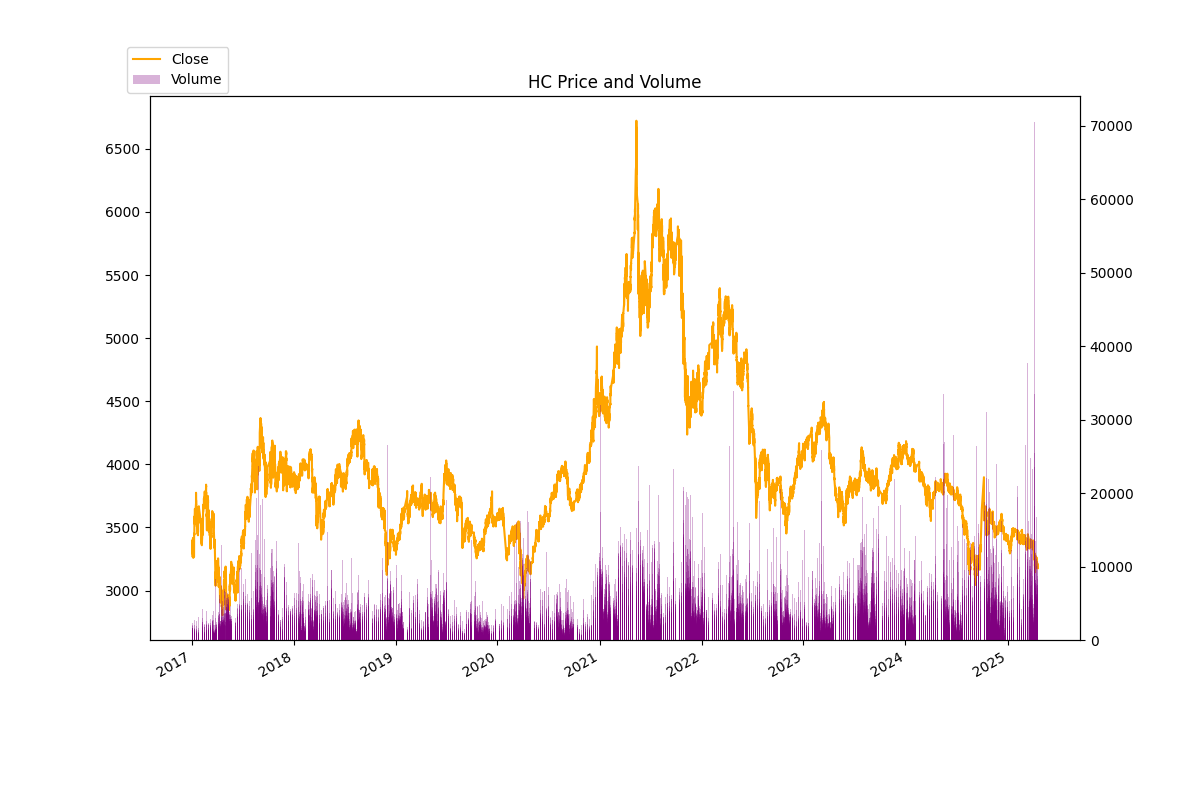
\includegraphics[width=\textwidth]{./v2/v0/HC.png}
  \caption*{异常值处理前HC的volume和close的重叠折线图}
  % \label{fig:drone_formation}
\end{figure}
\begin{figure}[H]
  \centering
  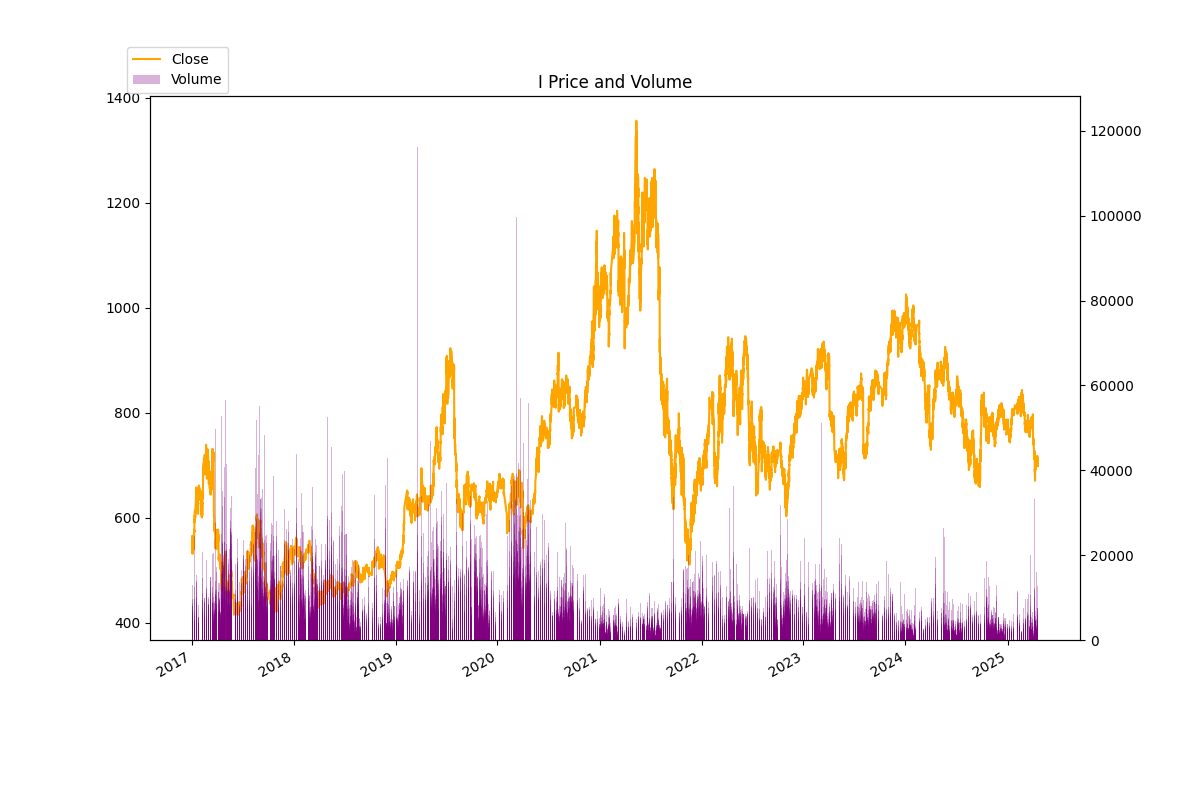
\includegraphics[width=\textwidth]{./v2/v0/I.png}
  \caption*{异常值处理前I的volume和close的重叠折线图}
  % \label{fig:drone_formation}
\end{figure}
\begin{figure}[H]
  \centering
  \includegraphics[width=\textwidth]{./v2/v0/JM.png}
  \caption*{异常值处理前JM的volume和close的重叠折线图}
  % \label{fig:drone_formation}
\end{figure}

% \newpage
\item 给出异常值处理后的close随时间变化的数值折线图:\FloatBarrier\noindent
\begin{figure}[H]
  \centering

    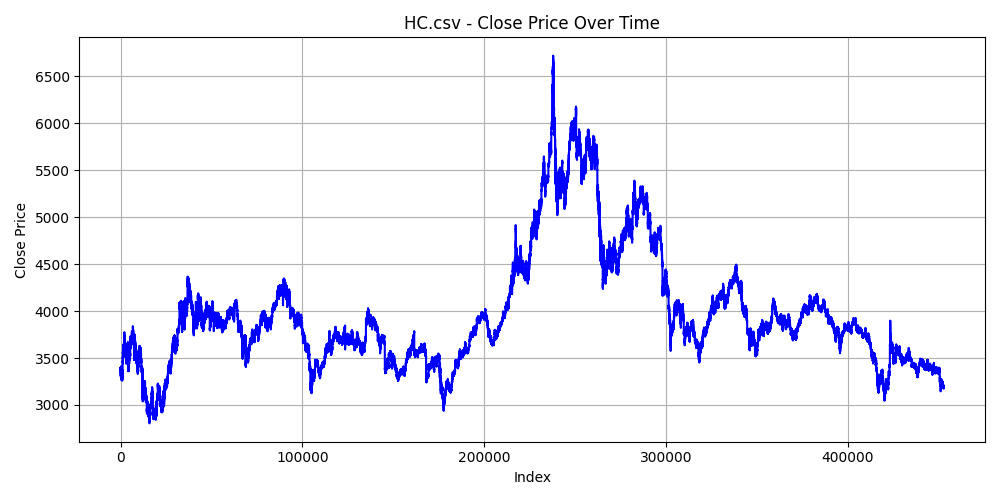
\includegraphics[width=\textwidth]{./v2/v2/HC.png}
    \caption*{异常值处理后HC的close的折线图}
\end{figure}


\begin{figure}[H]
  \centering

    \includegraphics[width=\textwidth]{./v2/v2/I.png}
    \caption*{异常值处理后I的close的折线图}
\end{figure}

  \begin{figure}[H]
  \centering

    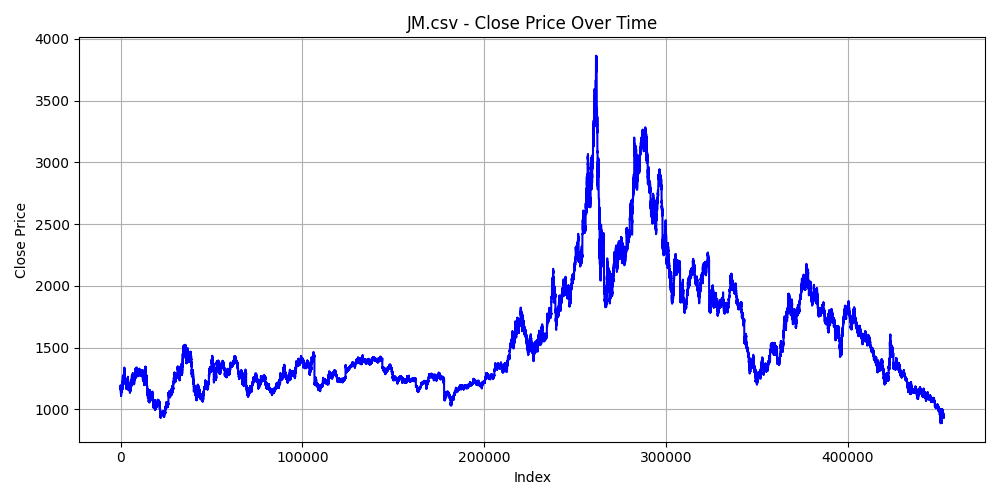
\includegraphics[width=\textwidth]{./v2/v2/JM.png}
    \caption*{异常值处理后JM的close的折线图}
  \end{figure}
  % 可以根据需要继续添加更多的子figure
  % \caption{整体图标题} % 如果需要为整个figure添加一个标题

\item 给出异常值处理后的volume对比图:\FloatBarrier\noindent
\begin{figure}[H]
  \centering

    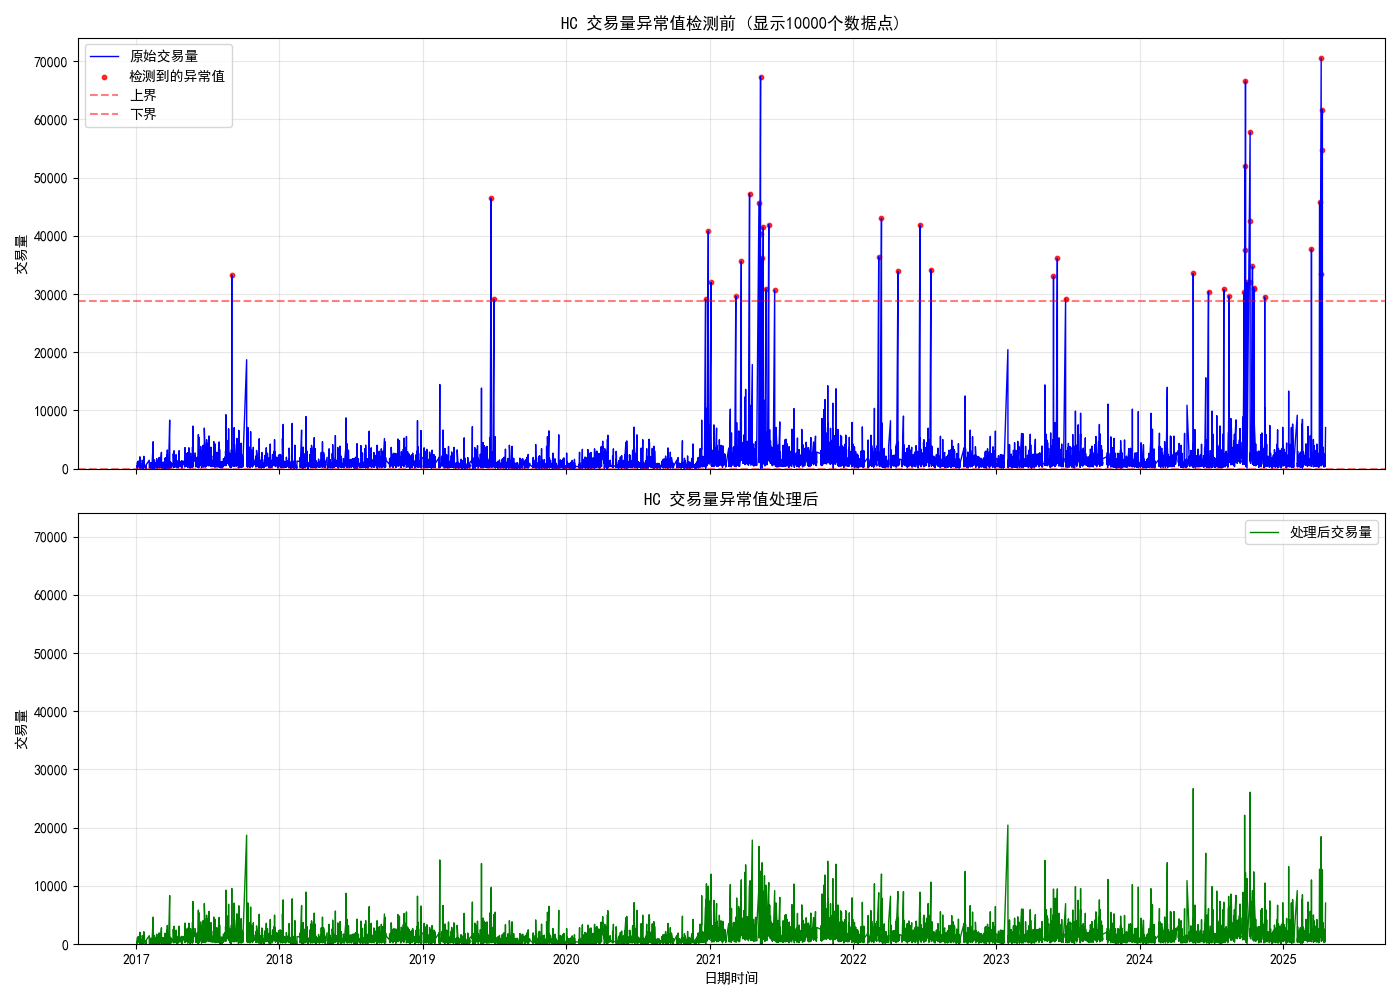
\includegraphics[width=\textwidth]{./v2/v3/HC.png}
    \caption*{异常值处理后HC的volume对比图}
  \end{figure}

  \begin{figure}[H]
    \centering
    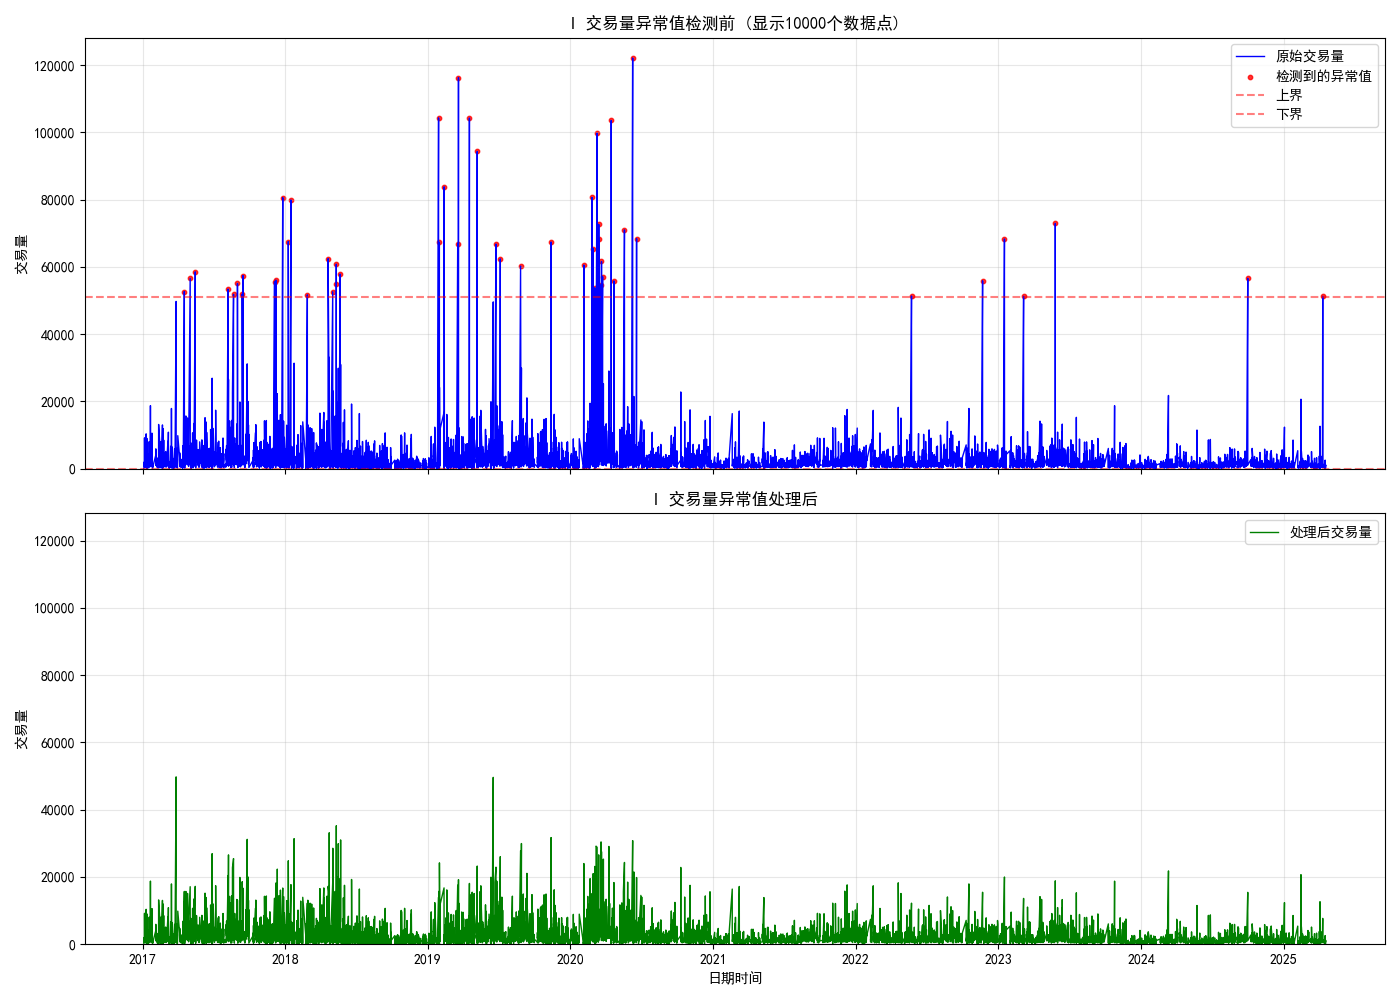
\includegraphics[width=\textwidth]{./v2/v3/I.png}
    \caption*{异常值处理后I的volume对比图}
  \end{figure}

  \begin{figure}[H]
    \centering
    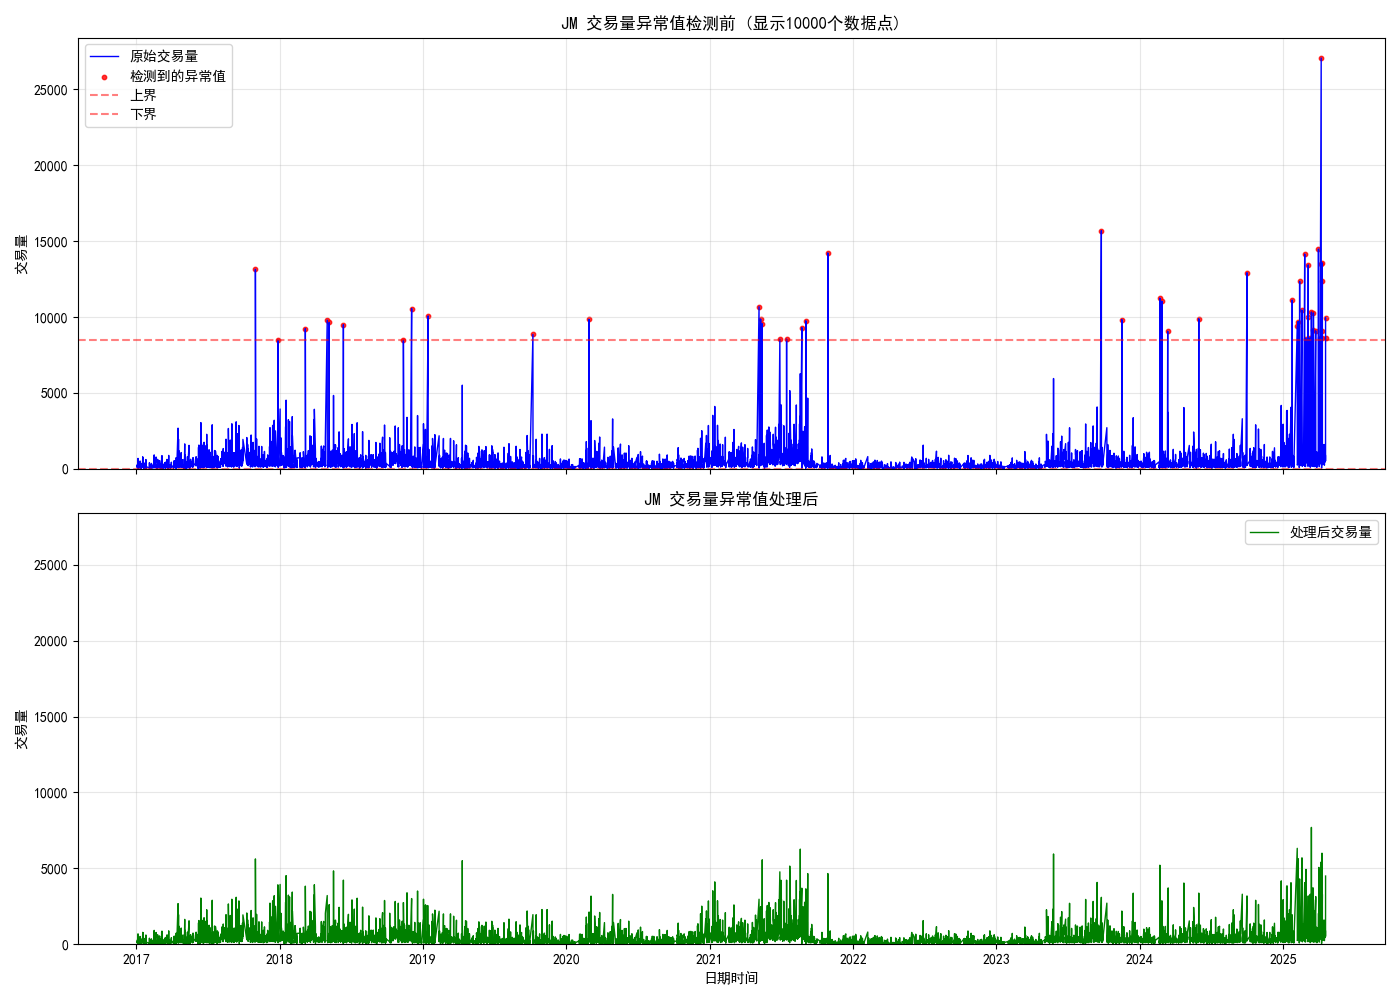
\includegraphics[width=\textwidth]{./v2/v3/JM.png}
    \caption*{异常值处理后JM的volume对比图}
  \end{figure}
  % 可以根据需要继续添加更多的子figure
  % \caption{整体图标题} % 如果需要为整个figure添加一个标题

\end{enumerate}
% \newpage
\subsection{特征提取}
提取和涨跌幅强相关的参数:

\begin{enumerate}
  \item 交易量随时间的变化率
  \item 交易量 volume 滞后 30 分钟和滞后 1 天的特征
  \item 交叉特征(波动率 $\times$ 交易量)
\end{enumerate}

\subsubsection{交易量随时间的变化率}

\paragraph{原理:}

交易量是市场活跃程度的重要指标。根据道氏理论和量价分析理论,价格变动若伴随交易量显著增长,则趋势更可能持续。交易量突增常伴随着主力资金的进出或情绪突变。

\paragraph{数学表达:}

交易量的变化率定义如下:
\[
\text{Volume Change Rate}_t = \frac{V_t - V_{t-1}}{V_{t-1}}*100\%
\]
其中 $V_t$ 表示当前时间点的交易量,$V_{t-1}$ 为上一个时间点的交易量。
% \FloatBarrier
% \noindent
% \begin{figure}[H]
%   \centering

%     \includegraphics[width=\textwidth]{./v3/交易量变化率/HC.png}
%     \caption*{HC的交易量变化率}
%   \end{figure}

%   \begin{figure}[H]
%     \centering
%     \includegraphics[width=\textwidth]{./v3/交易量变化率/I.png}
%     \caption*{I的交易量变化率}
%   \end{figure}

%   \begin{figure}[H]
%     \centering
%     \includegraphics[width=\textwidth]{./v3/交易量变化率/JM.png}
%     \caption*{JM的交易量变化率}
%   \end{figure}
  % 可以根据需要继续添加更多的子figure
  % \caption{整体图标题} % 如果需要为整个figure添加一个标题






\subsubsection{交易量滞后特征(30分钟和1天)}

\paragraph{原理:}

滞后交易量可以反映市场在过去某一时刻的活跃程度,有助于捕捉市场的短期记忆效应与行为惯性。30分钟滞后反映了短周期的交易节奏,1天滞后则体现了日内波动对次日走势的影响。

\paragraph{数学表达:}

令 $k$ 为滞后周期,则有:
\[
\text{Lagged Volume}_{t-k} = V_{t-k}
\]
常用的周期为 $k = 30\text{min},\ 1\text{d}$。

也可构造其相对变化:
\[
\Delta V_{t,k} = V_t - V_{t-k}, \quad \text{或} \quad \frac{V_t - V_{t-k}}{V_{t-k}}
\]

\subsubsection{交叉特征(波动率 $\times$ 交易量)}

\paragraph{原理:}

波动率和交易量是金融市场中两个重要且互补的指标。波动率衡量价格变动的幅度和频率,反映了市场的不确定性。高波动率通常意味着市场情绪不稳定,价格可能会出现大幅波动。相反,低波动率则表明市场相对平静,价格变动较小。交易量则反映了市场的活跃程度和资金流动情况。高交易量通常伴随着较大的市场情绪波动,表明有大量资金进出市场,可能预示着价格的显著变动。低交易量则表明市场较为冷清,价格变动可能较为温和。

通过将波动率与交易量结合,可以更全面地捕捉市场动态。交叉特征 ${Volatility \times Volume}$ 可以揭示市场剧烈波动前的征兆。具体来说,当波动率与交易量同时升高时,市场更可能出现大行情。这是因为高波动率和高交易量的结合通常意味着主力资金在市场中积极操作,市场情绪较为极端,从而可能导致价格的大幅波动。

此外,交叉特征还可以帮助识别市场的潜在趋势和拐点。在某些情况下,即使波动率较低,但如果交易量突然升高,也可能预示着即将出现的价格波动。反之,高波动率但低交易量可能意味着市场的不确定性,但缺乏足够的资金流动来驱动价格的显著变动。

\paragraph{数学表达:}

首先定义过去 $n$ 个时间点的波动率为:
\[
\text{Volatility}_t = \sqrt{\frac{1}{n} \sum_{i=t-n+1}^{t} (P_i - \bar{P})^2}
\]
其中 $P_i$ 表示第 $i$ 个时间点的价格,$\bar{P}$ 为该窗口内的平均价格。

交叉特征则为:
\[
\text{Volume-Volatility Interaction}_t = \text{Volatility}_t \times V_t
\]
\FloatBarrier
\noindent
  \begin{figure}[H]
  \centering

    \includegraphics[width=\textwidth]{./v3/交叉特征/HC.png}
    \caption*{HC的交叉特征}
  \end{figure}
  \begin{figure}[H]
    \centering
    \includegraphics[width=\textwidth]{./v3/交叉特征/I.png}
    \caption*{I的交叉特征}
  \end{figure}
  \begin{figure}[H]
    \centering
    \includegraphics[width=\textwidth]{./v3/交叉特征/JM.png}
    \caption*{JM的交叉特征}
 
  % 可以根据需要继续添加更多的子figure
  % \caption{整体图标题} % 如果需要为整个figure添加一个标题
  \end{figure}



\subsection{模型选择理由}

这是典型的监督学习 + 时间序列回归问题,特点是:

1.时间依赖性(前后时刻相关)

2.非线性特征影响(价格、成交量等复杂组合影响未来走势)\\

LSTM模型具备以下优势,利于实现这个任务:

1.记住较远历史信息

2.输入序列长度较长

3.输出依赖时间模式

4.输入输出为不定长序列\\

LSTM模型的数学-金融学背景如下:

\begin{itemize}
  \item[•] \textbf{门控机制的市场意义} \\
  LSTM 的门控机制天然适合捕捉期货市场的三类关键特征:

  \begin{table}[h]
  \centering
  \caption{LSTM门控与市场特征的对应关系}
  \begin{tabular}{lll}
  \toprule
  门控类型 & 数学表达 & 市场功能 \\
  \midrule
  遗忘门 & $\mathbf{f}_t=\sigma(\mathbf{W}_f[\mathbf{h}_{t-1},\mathbf{x}_t])$ & 过滤过时的技术指标 \\
   & & 衰减历史波动率影响 \\
  输入门 & $\mathbf{i}_t=\sigma(\mathbf{W}_i[\mathbf{h}_{t-1},\mathbf{x}_t])$ & 识别突破性行情 \\
   & & 吸收突发新闻事件 \\
  输出门 & $\mathbf{o}_t=\sigma(\mathbf{W}_o[\mathbf{h}_{t-1},\mathbf{x}_t])$ & 控制预测信号强度 \\
   & & 调节风险暴露程度 \\
  \bottomrule
  \end{tabular}
  \end{table}

  \item[•] \textbf{期货特征工程} \\
  输入特征设计为 5 维向量:
  \begin{equation*}
  \mathbf{x}_t = \begin{bmatrix}
  \frac{p_t - p_{t-5}}{p_{t-5}} & \text{(5分钟收益率)} \\
  \frac{\text{std}(p_{t-30:t})}{\text{mean}(p_{t-30:t})} & \text{(波动率)} \\
  \log(v_t/\bar{v}_{t-60}) & \text{(成交量偏离)} \\
  oi_t - oi_{t-30} & \text{(持仓量变化)} \\
  \mathbb{I}_{\text{夜盘时段}} & \text{(交易时段标记)}
  \end{bmatrix}
  \end{equation*}

  \item[•] \textbf{梯度传播的市场解释}
  \begin{center}
  \begin{minipage}[t]{0.6\linewidth}
  \begin{equation*}
  \frac{\partial \mathcal{L}}{\partial \mathbf{C}_{t-1}} = \mathbf{f}_t + \frac{\partial}{\partial \mathbf{C}_{t-1}}(\mathbf{i}_t \odot \tilde{\mathbf{C}}_t)
  \end{equation*}
  \end{minipage}
  \begin{minipage}[t]{0.35\linewidth}
  \begin{itemize}
    \item 趋势市中 $\mathbf{f}_t \approx 1$
    \item 震荡市中 $\mathbf{i}_t$ 主导更新
    \item 极端行情时梯度爆炸抑制
  \end{itemize}
  \end{minipage}
  \end{center}

  \item[•] \textbf{改进的 Peephole 结构}
  \begin{equation*}
  \begin{aligned}
  \mathbf{f}_t &= \sigma\left(\mathbf{W}_f[\mathbf{C}_{t-1}, \Delta p_{t-1}] + \mathbf{b}_f\right) \\
  \mathbf{o}_t &= \sigma\left(\mathbf{W}_o[\mathbf{C}_t, \text{VIX}_t] + \mathbf{b}_o\right)
  \end{aligned}
  \end{equation*}
  \begin{itemize}
    \item 价格加速度 $\Delta p_{t-1}$ 增强趋势判断
    \item VIX 指数调节风险控制强度
  \end{itemize}
\end{itemize}




% \newpage
\subsection{模型具体实现} 

模型实现结构图全览:

\begin{center}
\scalebox{0.85}{ % 整体缩放
\tikzset{
  block/.style={rectangle, draw, text centered, minimum height=1.8em, minimum width=3em, rounded corners, font=\small},
  oval/.style={ellipse, draw, minimum height=1.8em, minimum width=4em, text centered, font=\small},
  arrow/.style={-Stealth, thick, shorten >=2pt, shorten <=2pt},
  box/.style={draw, thick, dashed, inner sep=0.2cm, rounded corners, font=\footnotesize}
}

\begin{tikzpicture}[node distance=0.8cm and 0.6cm]

% --- Preprocess Block ---
\node[oval] (data) {Data};

\node[block, below left=0.6cm and 0.5cm of data] (scaler) {MinMaxScaler};
\node[block, below=0.6cm of data] (cleaner) {Cleaner};
\node[block, below right=0.6cm and 0.5cm of data] (dataset) {TS Dataset};

\draw[arrow] (data) -- (scaler);
\draw[arrow] (data) -- (cleaner);
\draw[arrow] (data) -- (dataset);

\node[box, fit=(scaler)(cleaner)(dataset), label=below:Preprocess] (prebox) {};

% --- LSTM Module ---
\node[oval, below=1.2cm of cleaner] (lstm) {LSTM};
\draw[arrow] (cleaner) -- (lstm);

% Input Model
\node[oval, left=2.2cm of lstm] (input_model) {Input};
\node[block, below=0.6cm of input_model] (bn1) {BN};

\draw[arrow] (lstm) -- (input_model);
\draw[arrow] (input_model) -- (bn1);

% LSTM Layers
\node[oval, below=1cm of lstm] (lstmer) {LSTMer};
\node[block, below=0.6cm of lstmer] (lstm1) {LSTM64};
\node[block, below=0.6cm of lstm1] (drop1) {Drop0.3};
\node[block, below=0.6cm of drop1] (lstm2) {LSTM32};
\node[block, below=0.6cm of lstm2] (drop2) {Drop0.3};

\draw[arrow] (lstm) -- (lstmer);
\draw[arrow] (lstmer) -- (lstm1);
\draw[arrow] (lstm1) -- (drop1);
\draw[arrow] (drop1) -- (lstm2);
\draw[arrow] (lstm2) -- (drop2);

% Output Model
\node[oval, right=2.2cm of lstm] (output_model) {Output};
\node[block, below=0.6cm of output_model] (linear1) {Linear16};
\node[block, below=0.6cm of linear1] (bn2) {BN};
\node[block, below=0.6cm of bn2] (relu) {ReLU};
\node[block, below=0.6cm of relu] (drop3) {Drop0.15};

\draw[arrow] (lstm) -- (output_model);
\draw[arrow] (output_model) -- (linear1);
\draw[arrow] (linear1) -- (bn2);
\draw[arrow] (bn2) -- (relu);
\draw[arrow] (relu) -- (drop3);

% Merge Output
\node[block, below=1.5cm of drop2] (linear2) {Linear1};
\node[oval, below=0.6cm of linear2] (output_final) {Output};

\draw[arrow] (drop2) -- (linear2);
\draw[arrow] (drop3) -- (linear2);
\draw[arrow] (linear2) -- (output_final);

\node[box, fit=(input_model)(bn1)(lstmer)(drop2)(output_model)(drop3), label=below:Network] (netbox) {};
\end{tikzpicture}
}
\end{center}


模型实现结构分层次剖析:

\subsubsection{数据预处理}
\begin{itemize}
  \item[1.] \textbf{数据标准化} \\
  采用 Min-Max 标准化处理原始期货数据:
  \begin{equation}
  x_{\text{scaled}} = \frac{x - \min(X)}{\max(X) - \min(X)} \quad \text{(将特征缩放到 [0,1] 区间)}
  \end{equation}

  \item[2.] \textbf{数据清洗}
  \begin{itemize}
    \item 处理缺失值:前向填充(Forward Fill)
    \item 异常值处理:剔除 $\pm 3\sigma$ 外的价格数据
    \item 跳空修复:对隔夜缺口进行线性插值
  \end{itemize}

  \item[3.] \textbf{时序数据集构建} \\
  构建监督学习格式的时序数据:
  \begin{equation}
  \mathcal{D} = \{ (\mathbf{X}_t, y_t) \mid \mathbf{X}_t = [\mathbf{x}_{t-T}, ..., \mathbf{x}_t], \ y_t = p_{t+30} \}
  \end{equation}
  其中 $T=120$ 表示 2 小时历史窗口(对应图中 TimeSeries Dataset)
\end{itemize}


\subsubsection{网络架构}

\begin{itemize}
\item \textbf{输入特征}:包含交易量变化率,交易量滞后特征,交叉特征3个维度,经标准化处理后输入网络

\item \textbf{核心组件}:
  \begin{itemize}
  \item \textbf{BatchNorm层}:对输入特征进行归一化,设置$\epsilon=10^{-5}$防止数值不稳定
  \item \textbf{双层LSTM结构}:
    \begin{itemize}
    \item 第一层:64维隐藏状态,捕捉短期波动模式
    \item 第二层:32维隐藏状态,提取高阶时序特征
    \end{itemize}
  \item \textbf{Dropout层}:
    \begin{itemize}
    \item 第一层丢弃率0.3,缓解市场噪声影响
    \item 第二层丢弃率0.15,保留有效特征
    \end{itemize}
  \end{itemize}

\item \textbf{输出层设计}:
  \begin{itemize}
  \item 通过16维全连接层压缩特征
  \item ReLU激活保证预测收益率非负
  \item L2正则化($\lambda=0.01$)控制模型复杂度
  \end{itemize}
\end{itemize}


% \newpage



\subsection{模型的训练与验证}
\subsubsection{数据预处理流程}
\begin{itemize}
\item \textbf{异常值处理}:
  \begin{itemize}
  \item 采用前向填充与线性插值组合策略:
    \[
    x_t^{\text{filled}} = \begin{cases}
    x_{t-1} & \text{单点缺失} \\
    \text{linear}(x_{t-k}, x_{t+m}) & \text{连续缺失}
    \end{cases}
    \]
  \item 剔除$\pm 3\sigma$外的极端值,保留市场正常波动范围
  \end{itemize}
  
\item \textbf{特征工程}:
  \begin{itemize}
  \item 动态缩放:对每个特征列独立进行MinMax标准化
    \[
    x^{(j)} \leftarrow \frac{x^{(j)} - \min(X^{(j)})}{\max(X^{(j)}) - \min(X^{(j)})}
    \]
  \item 状态保存:持久化scaler参数供生产环境复用
  \end{itemize}
\end{itemize}


\subsubsection{优化训练策略}
\begin{figure}[h]
\centering
\begin{tikzpicture}[node distance=1cm, auto]
\node (train) {训练epoch};
\node (loss) [right=of train] {计算复合损失};
\node (clip) [right=of loss] {梯度裁剪};
\node (update) [right=of clip] {参数更新};
\node (val) [below=of update] {验证评估};
\node (lr) [left=of val] {学习率调整};
\node (stop) [left=of lr] {早停判断};
\path[->] 
(train) edge (loss)
(loss) edge (clip)
(clip) edge (update)
(update) edge (val)
(val) edge (lr)
(lr) edge (stop);
\end{tikzpicture}
\caption{训练循环控制流}
\end{figure}

关键组件:
\begin{itemize}
\item \textbf{自适应优化器}:采用AdamW(改进版Adam):
  \begin{itemize}
  \item $\beta_1=0.9,\ \beta_2=0.999$ 平衡短期动量与长期方差
  \item 解耦权重衰减实现更稳定的L2正则
  \end{itemize}
  
\item \textbf{动态学习率}:ReduceLROnPlateau调度器:
  \[
  \eta \leftarrow \begin{cases}
  0.5\eta & \text{Val MSE连续5轮$\nrightarrow$} \\
  \eta & \text{otherwise}
  \end{cases}
  \]
  
\item \textbf{损失函数}:
  \[
  \mathcal{L} = \underbrace{\frac{1}{N}\sum(y-\hat{y})^2}_{\text{MSE}} + \lambda \underbrace{\|\mathbf{W}\|_2^2}_{\text{L2}} + \alpha \underbrace{\|\mathbf{h}_t-\mathbf{h}_{t-1}\|_2^2}_{\text{状态平滑}}
  \]

  \item \textbf{过拟合处理}:

  \begin{itemize}
  \item \textbf{L2正则化}:
    \[
    \mathcal{L}_{reg} = \lambda\sum w_i^2 \quad (\lambda=0.01)
    \]
    通过AdamW优化器实现解耦权重衰减
    
  \item \textbf{Dropout策略}:
    \begin{itemize}
    \item 第一层LSTM后:0.3丢弃率过滤噪声
    \item 第二层LSTM后:0.15丢弃率保留有效特征
    \end{itemize}
  
  \item \textbf{梯度约束}:
    \[
    \mathbf{g} \leftarrow \min\left(1.0, \frac{1.0}{\|\mathbf{g}\|_2}\right)\mathbf{g}
    \]
    特别应对交割月合约的剧烈波动
  
  
  \item \textbf{早停机制}:
  \begin{itemize}
  \item 基于验证集MSE的patience=10策略
    \item 保留最佳模型状态:选择验证集均方误差最小对应的参数 $\mathbf{W}_{\text{best}}$,即
        \[
        \mathbf{W}_{\text{best}} = \min_{\mathbf{W}} \text{MSE}_{\text{val}}(\mathbf{W})
        \]
  \end{itemize}
  \end{itemize}
  
  
  \item \textbf{SMA数据增强}:
    \begin{itemize}
    \item \textbf{多周期移动平均}:
      \begin{align*}
      \text{SMA}_{20} &= \frac{1}{20}\sum_{i=0}^{19} p_{t-i} \\
      \text{SMA}_{60} &= \frac{1}{60}\sum_{i=0}^{59} p_{t-i} \\
      \text{EMA}_{10} &= 0.18p_t + 0.82\text{EMA}_{10}(p_{t-1})
      \end{align*}
      
    \item \textbf{衍生特征构建}:
      \begin{equation*}
      \begin{aligned}
      \text{Price-SMA20 Ratio} &= \frac{p_t}{\text{SMA}_{20}} - 1 \\
      \text{SMA20-SMA60 Delta} &= \text{SMA}_{20} - \text{SMA}_{60} \\
      \text{EMA10 Slope} &= \text{EMA}_{10}(p_t) - \text{EMA}_{10}(p_{t-5})
      \end{aligned}
      \end{equation*}
      
    \item \textbf{金融逻辑}:
      \begin{itemize}
      \item 价格/均线比率识别超买超卖状态
      \item 双均线差值判断趋势强度
      \item EMA斜率捕捉短期动量变化
      \end{itemize}
    \end{itemize}
  \end{itemize}
  
\subsubsection{验证与模型选择}
\begin{itemize}
\item \textbf{双重评估指标}:
  \begin{align*}
  \text{MSE} &= \frac{1}{N}\sum(y_i-\hat{y}_i)^2 \quad \text{(强调极端误差)} \\
  \text{MAE} &= \frac{1}{N}\sum|y_i-\hat{y}_i| \quad \text{(衡量平均偏差)}
  \end{align*}
  

\item \textbf{交叉验证}:时序分割(TimeSeriesSplit)保持时间依赖
\end{itemize}

\subsubsection{实现优化亮点}
\begin{itemize}
\item \textbf{内存管理}:
  \begin{itemize}
  \item DataLoader的pin\_memory加速GPU数据传输
  \item 梯度累积支持超大batch size
  \end{itemize}
  
\item \textbf{可复现性}:
  \begin{itemize}
  \item 设置全局随机种子(seed=42)
  \item 确定性算法配置
  \end{itemize}
  
\item \textbf{生产部署}:
  \begin{itemize}
  \item 模型量化(FP16)提升推理速度
  \item 异常输入自动检测与恢复
  \end{itemize}
\end{itemize}
\subsubsection{模型训练及验证结果}
使用回归问题中常见的MSE均方误差和MAE平均绝对误差作为评价标准

选择HC,JM,RB三种期货进行可视化如下图

HC和JM在训练轮次到达4轮左右时, 误差接近收敛

RB的验证集平均绝对误差呈波动下降, 没有出现过拟合和欠拟合的情况, 效果最优
\FloatBarrier
\noindent
\begin{figure}[H]
  \centering
  \includegraphics[width=\textwidth]{./pic/HC_train.png}
  \caption*{HC模型训练曲线}
  % \label{fig:drone_formation}
\end{figure}
\begin{figure}[H]
  \centering
  \includegraphics[width=\textwidth]{./pic/JM_train.png}
  \caption*{JM模型训练曲线}
  % \label{fig:drone_formation}
\end{figure}
\begin{figure}[H]
  \centering
  \includegraphics[width=\textwidth]{./pic/RB_train.png}
  \caption*{RB模型训练曲线}
  % \label{fig:drone_formation}
\end{figure}




\subsection{模型预测效果与改进建议}
\subsubsection{模型训练及验证结果}
先根据模型计算出预测的收盘价close和实际收盘价做对比, 可视化展示发现误差在可控范围内
\begin{figure}[H]
  \centering
  \includegraphics[width=\textwidth]{./pic/RB_compare.png}
  \caption*{RB收盘价预测与模型的对比}
  % \label{fig:drone_formation}
\end{figure}

计算得到最终所需的涨跌幅数据, 展示其中3种期货的可视化图片
\FloatBarrier
\noindent
\begin{figure}[H]
  \centering
  \includegraphics[width=\textwidth]{./pic/HC_change.png}
  \caption*{HC涨跌幅预测}
  % \label{fig:drone_formation}
\end{figure}
\begin{figure}[H]
  \centering
  \includegraphics[width=\textwidth]{./pic/SM_change.png}
  \caption*{SM涨跌幅预测}
  % \label{fig:drone_formation}
\end{figure}
\begin{figure}[H]
  \centering
  \includegraphics[width=\textwidth]{./pic/SS_change.png}
  \caption*{SS涨跌幅预测}
  % \label{fig:drone_formation}
\end{figure}



预测的各期货涨跌幅评估指标:
\begin{table}[H]
  \centering
  \caption{各期货品种预测性能对比}
  \begin{tabular}{|c|c|c|} 
    \hline
    \textbf{期货品种} & \textbf{方向预测准确率(\%)} & \textbf{涨跌幅MAE(\%)} \\
    \hline
    HC & 65.45 & 0.37 \\
    \hline
    SS & 64.72 & 0.35 \\
    \hline
    SF & 66.31 & 0.32 \\
    \hline
    SM & 61.26 & 0.29 \\
    \hline
    RB & 68.18 & 0.33 \\
    \hline
    I & 67.54 & 0.33 \\
    \hline
    JM & 64.88 & 0.34 \\
    \hline
  \end{tabular}
  \label{tab:prediction_performance}
\end{table}

\subsubsection{模型改进建议}
未来研究可从以下几个方向进行改进:\\
(1)引入市场情绪和宏观经济指标等外部特征,提升模型对市场转折点的敏感度;\\
(2)探索注意力机制和更先进的神经网络架构如Transformer,增强模型对长期依赖的捕捉能力;\\
(3)结合强化学习技术,直接优化交易决策而非单纯预测涨跌幅;\\
(4)开发更具解释性的模型结构,帮助投资者理解预测背后的市场逻辑。\\

\newpage
\section{参考文献}
\renewcommand\refname{} % 禁用 bibliography 默认标题(article 类)
\begin{thebibliography}{9}

\bibitem{he2004}
何光辉. 处理金融时间序列的非平稳性和时变性——2003年诺贝尔经济学奖得主的理论贡献[J]. 国际金融研究, 2004(5): 74–78.

\bibitem{zhao2021}
赵婷婷, 韩雅杰, 杨梦楠, 任德华, 陈亚瑞, 刘建征. 基于机器学习的时序数据预测方法研究综述[J]. 天津科技大学学报, 2021, 36(5): 1–9.

\bibitem{wang2007}
王永民, 何幼桦, 忻莉莉, 王巧兰. 时变自回归模型系数的估计及预测[J]. 应用数学与计算数学学报, 2007, 21(2): 35–41.

\bibitem{onlstm}
Shen Y, Tan S, Sordoni A, Courville A. Ordered Neurons: Integrating Tree Structures into Recurrent Neural Networks[EB/OL]. arXiv preprint arXiv:1810.09536v6, 2018. Available: \url{http://arxiv.org/pdf/1810.09536v6}.

\bibitem{lrcn}
Donahue J, Hendricks L A, Rohrbach M, Venugopalan S, Guadarrama S, Saenko K, Darrell T. Long-Term Recurrent Convolutional Networks for Visual Recognition and Description[J]. IEEE Transactions on Pattern Analysis and Machine Intelligence, 2017, 39(4): 677–691. DOI: \href{https://doi.org/10.1109/TPAMI.2016.2599174}{10.1109/TPAMI.2016.2599174}.

\bibitem{latticelstm}
Zhang Y, Yang J. Chinese NER Using Lattice LSTM[C]// Proceedings of the 56th Annual Meeting of the Association for Computational Linguistics (Volume 1: Long Papers), 2018: 1554–1564. 

\bibitem{convlstm}
Shi X, Chen Z, Wang H, Yeung D Y, Wong W K, Woo W C. Convolutional LSTM Network: A Machine Learning Approach for Precipitation Nowcasting[C]// Advances in Neural Information Processing Systems (NeurIPS), 2015, 28: 802–810.

\end{thebibliography}

\iffalse
\section{源码与文档}
预处理部分:
preprocess.py 对原始数据进行预处理 \\
OutlierClean.py volume异常值处理 \\
特征提取部分:
feature_extract_volume.py 提取交易量变化率 \\
lag_feature.py 提取交易量滞后特征 \\
cross_feature.py 提取交叉特征 \\
模型训练与验证部分:
train.py \\
模型预测与评估部分:
predict.py \\
\fi

\end{document}